\chapter{Zastosowanie systemów mrówkowych w steganografii}\label{chap:stegoants}
{
    % - wstęp
    %   - skoro mrówki mają tak szerokie zastosowania, to czemu nie użyć ich w steganografii?
    %   - jaki jest główny cel oraz problem steganografii? (jakoś obrazu jest odwrotnie proporcjonalna do ilości
    %     ukrytych informacji)
    %   - pomysł: odpowiedni dobór miejsc w których zostaną ukryte informacje (wykorzystanie `complex` regions)
    %   - zalety: stochastyczność procesu (bezpieczeństwo++)
    % - coś powiedzieć o zasadzie Kerckhoffsa i dodatkowym bezpieczeństwie z nią związaną
    % - przytoczenie (krótkie) istniejących prac, ich założeń/wad/zalet
    %  moja metoda:
    % - kwestia reprezentacji obrazu jako grafu
    %   - czym są węzły
    %   - czym są krawędzie
    %   - jak wyznaczono długości krawędzi
    % - modyfikacje zasad działania systemu mrówkowego aby przystosować go do problemu
    %   - brak pełnych cykli (ograniczenie ilości kroków)
    % - interpretacja śladu feromonowego
    %   - metody przekształceń (tzn ograniczenie zakresu wartości, skalowanie itp)

    Jak przedstawiono w poprzednich rozdziałach, zagadnienia steganografii oraz systemów mrówkowych są złożone, nawet
    gdy są analizowane w izolacji. Obie dziedziny mogą zostać powiązane, jeśli będą rozpatrywane jako parę problemu
    optymalizacji oraz metaheurystykę mogącą posłużyć do jego rozwiązania.

    % GŁÓWNY PROBLEM: ILOŚĆ vs JAKOŚĆ
    Wykorzystanie systemów steganograficznych jest bezpośrednio związane z jednoczesną realizacją celów stojących w
    opozycji. Idealny system steganograficzny, niezależnie od stosowanego medium nośnego, cechuje się jednocześnie dużą
    pojemnością, odpornością na zakłócenia i zniekształcenia nośnika i niską wykrywalnością istnienia przekazu.
    Intuicyjnie, lecz również na podstawie wszelkich obserwacji, można zauważyć że jednoczesna maksymalizacja ukrywanego
    przekazu powoduje wzrost cech niepożądanych, takich jak wzrost podatności na ataki steganograficzne. Oznacza to, że
    kluczowym aspektem wszystkich metod steganograficznych jest zachowanie balansu pomiędzy realizacją tych celów. W
    zastosowaniach o krytycznej poufności istotniejsze będzie zapewnienie niższej wykrywalności, nawet jeśli się
    odbędzie kosztem stosunku wiadomości do sygnału. W zależności od wybranej metody, kontrolowanie tego balansu może
    się to sprowadzać do regulacji parametrów algorytmu lub wyboru nośnika o odpowiednio dużym rozmiarze.

    % METODY HEURYSTYCZNE - ZALETY W STEGANOGRAFII
    \section{Zastosowanie metod heurystycznych w steganografii}\label{sec:heuristics-ants}
    {
        Trudności związane z optymalizacją procesu nie oznaczają, że należy zaniechać poszukiwań metod pozwalających na
        zachowanie zadowalającego poziomu każdego z parametrów procesu. W rzeczywistości, zagadnienie wykorzystania
        metaheurystyk oraz metod uczenia maszynowego do celów steganografii jest aktywną dziedziną odnoszącą ciągłe
        sukcesy \cite{ElEmam2013NewSA, Zhao2021AntCO, Khan2018AntCO, Saleema2016ANS, Li2007ASM}.
        % STOSOWANIE KLUCZY
        Jednym z aspektów przemawiających na korzyść stosowania metod heurystycznych do celów steganograficznych jest
        ich stochastyczny charakter. Podstawowym problemem najprostszych technik steganograficznych, takich jak
        \textit{LSB}, jest sekwencyjny wybór fragmentów nośnika informacji. W przypadku ukrywania informacji w
        obrazach, najoczywistszym działaniem jest kodowanie danych w kolejnych pikselach obrazu. Takie podejście jest
        wyjątkowo podatne na najprostsze formy ataków, zarówno steganograficznych jak i statystycznych. W celu
        uniknięcia powyższej podatności, możliwe jest stosowanie dodatkowych kluczy instruujących, które i w jakiej
        kolejności segmenty nośnika należy analizować \cite{AlHusainy2019ASI}. Wykorzystanie stochastycznych procesów
        które zachodzą w znacznej części metaheurystyk, automatycznie rozwiązuje problem przewidywalności umiejscowienia
        informacji. Gwarantuje również możliwość powtarzalnego odtworzenia jego działania poprzez ustalanie ziarna
        generatora liczb losowych. W takim przypadku, jego wartość stanowi swoisty klucz zwiększający bezpieczeństwo
        ukrytych danych.
        % ZASADA KERCKHOFFSA
        Dodatkowym argumentem przemawiającym za słusznością wykorzystania klucza w metodach steganograficznych, jest
        słynna zasada Kerckhoffsa \cite{Guillot2013AugusteKE}, będąca fundamentem współczesnej kryptografii. Jej treść
        głosi, że bezpieczeństwo systemu powinno zostać zachowane, nawet jeśli osoba próbująca odkryć poufne informacje
        zna wszystkie szczegóły jego działania. Gwarantem bezpieczeństwa musi być prywatny klucz. Zasada ta stoi w
        opozycji do systemów opierających się na niejawności \textit{(ang. Security by obscurity)}.

        % SYSTEMY MRÓWKOWE W STEGANOGRAFII
        \subsection{Systemy mrówkowe w steganografii}
        {
            W związku z zaletami metod heurystycznych, oraz nadziejami na znalezienie sposobu optymalizacji
            przeciwstawnych cech steganogramów, próby wykorzystania systemów mrówkowych i mrowiskowych do ukrywania
            danych w obrazach były niejednokrotnie podejmowane \cite{Priya2018HIGHCA, ZghaerACOStegEN, Khan2018AntCO}.
            % REPREZENTACJA PROBLEMU + INTERPRETACJA WYNIKÓW
            Najważniejszym aspektem charakteryzującym każdą z opisanych metod jest sposób reprezentacji problemu. W celu
            zastosowania metaheurystyki systemu mrówkowego, konieczne jest przedstawienie danych wejściowych w postaci
            grafu. Wybór dotyczący zasady jego budowy ma fundamentalny wpływ na uzyskiwane rezultaty oraz efektywność
            algorytmu. Kolejnym kluczowym zagadnieniem jest interpretacja rezultatów pracy wirtualnych mrówek. W tej
            kwestii istnieją conajmniej dwie obierane ścieżki przez eksperymentatorów. Za wynik działania algorytmu
            można uznać najkrótszą bądź najpopularniejszą ścieżkę obieraną przez mrówki -- takie podejście oznacza
            pozyskanie dyskretnej listy wykorzystanych krawędzi. Alternatywnie, jako rezultat można uznać utworzony ślad
            feromonowy. Korzystając z tego podejścia, wynikiem działania algorytmu jest zbiór rozmyty krawędzi
            reprezentujących najlepszą ścieżkę -- krawędzie częściej należące do krótszych rozwiązań problemu
            komiwojażera będą bardziej do niego należeć niż ścieżki rzadko obierane. Analiza zbioru rozmytego rozwiązań
            pozostawia szerszą możliwość interpretacji wyników. Dodatkowo, charakterystyka uzyskiwanego śladu
            feromonowego jest bardziej podatna na zmiany rodzaju systemu mrówkowego oraz jego parametry.

            % PRZYKŁD - CZĘSTOTLIWOŚCIOWO
            Systemy mrowiskowe mogą zostać wykorzystane zarówno w steganografii za pomocą obrazów cyfrowych w dziedzinie
            przestrzennej  \cite{ZghaerACOStegEN, Khan2018AntCO}, jak i częstotliwościowej \cite{Priya2018HIGHCA}. W
            artykule \cite{Priya2018HIGHCA}, zaproponowano metodę opartą na przytoczonej metodzie całkowitoliczbowej
            transformaty falkowej (\textit{IWT}). Twórcy opisali algorytm wykorzystujący system mrowiskowy do ukrycia
            sekretnej informacji w współczynnikach dziedziny transformaty. Przeprowadzone eksperymenty wykazały wysoką
            skuteczność metody \cite{Priya2018HIGHCA}.

            % PRZYKŁD - PRZESTRZENNIE
            Pomimo że pozostałe przytoczone prace oparte są na analizie obrazu w technice przestrzennej, sposób
            reprezentacji problemu i interpretacji wyników jest zdecydowanie odmienny. W pracy ,,Ant Colony
            Optimization To Enhance Image Steganography'' \cite{ZghaerACOStegEN}, obrazy zostały podzielone na bloki o
            rozmiarach $2 \times 2$ lub $5 \times 5$. Każdy blok jest interpretowany jako graf, w którym wierzchołkami
            są piksele, a długościami krawędzi są odwrotności błędu średniokwadratowego spowodowanego przez ukrycie w
            danym pikselu jednego bitu informacji. Uzyskana przez system mrówkowy ścieżka wskazuje, w których pikselach
            należy umieścić informację aby uzyskać najmniejszy wpływ na różnicę między obrazem nośnym a
            stganogramem \cite{ZghaerACOStegEN}.

            % PRZYKŁD - PRZESTRZENNIE 2
            Przykładem pracy wykorzystującej wartości śladu feromonowego naniesionego przez mrówki jest ,,Ant Colony
            Optimization (ACO) based Data Hiding in Image Complex Region'' \cite{Khan2018AntCO}. W powyższej pracy,
            mrówki poruszają się po grafie zbudowanym na podstawie bitmapy nośnej. Jego wierzchołkami są piksele, a
            długościami krawędzi różnice intensywności pikseli przez nie łączone. Dążeniem stosowania takiej
            reprezentacji jest wykrycie krawędzi oraz złożonych obszarów obrazu, pozwalających na ukrycie większej
            ilości informacji przy jednoczesnej niższej wykrywalności ingerencji w obraz. Po ukończeniu pracy systemu
            mrowiskowego, ustalana jest wartość graniczna feromonu, dla której piksele uznawane są za należące do
            złożonego segmentu. W ten sposób, obraz zostaje podzielony na dwa zbiory pikseli. W tych związanych z
            wartością feromonu przekraczającą wartość graniczną zostaje stosowana technika \textit{LSB}. Pozostałe
            piksele pozostają niezmienione. Za pomocą wyników eksperymentów udało się dowieźć że jest to skuteczna
            metoda. Jej dodatkową zaletą jest możliwość parametryzacji i zmiany sposobu wyznaczania granicznej wartości
            feromonu, co pozwala na sterowanie pojemnością steganogramu kosztem jakości \cite{Khan2018AntCO}.
        }
    }
    % wady/zalety powyższych podejść, czego nie zbadały lub co można było ulepszyć 
    %
    % przytoczenie zasad sugerujących korzystanie z complex region
    % przytoczenie metod vLSB i podobnych
    % zaproponować 2 inne podejścia reprezentacji grafu + sposoby interpretacji śladu feromonowego z nimi związane

    \section{Zaproponowana metoda}\label{sec:assumptions}
    {
        Przytoczone i opisane metody udowadniają użyteczność i skuteczność wykorzystania systemów mrówkowych w celach
        steganograficznych. Jednocześnie, przegląd dostępnej literatury sugeruje że nie jest to temat wyczerpany, a jego
        dalsza eksploracja jest możliwa i niesie nadzieję na odkrycie metod jeszcze lepszych pod kątem pojemności
        steganogramu i niższej postrzegalności przekazu. Poniżej przytoczono główne założenia i idee dwóch badanych
        metod wykorzystujących systemy mrówkowe i mrowiskowe do ukrywania informacji w obrazach w celu zapewnienia
        możliwie najwyższej jakości steganogramu i jego pojemności.

        % IDEA DOBORU REGIONU OBRAZU: ZŁOŻONOŚĆ + STOCHASTYCZNOŚĆ
        \subsection{Założenia}
        {
            Pierwszą decyzją podjętą podczas projektowania rozwiązania problemu było zdecydowanie się na wykorzystanie
            sekcji obrazów cechujących się większą złożonością, takich jak krawędzie i zróżnicowane tekstury. Istniejąca
            literatura z dziedziny steganografii sugeruje wyższą podatność na manipulację w takich właśnie obszarach
            przy zachowaniu jednoczesnej niskiej postrzegalności istnienia przekazu. Przykładem powszechnie przyjętej
            techniki opartej na powyższej tezie jest opisana w rozdziale \ref{chap:steganography} metoda \textit{Value
            Pixel Differencing \textnormal{(}VPD\textnormal{)}} \cite{Wu2003ASM}, polegająca na uzależnieniu liczby
            wykorzystanych bitów od miary różnicy sąsiadujących pikseli. Poparcia powyższej tezy można również szukać w
            przykładach metod opartych na dziedzinie częstotliwościowej obrazu \cite{Xuan2005LosslessDH}.

            % METODA UKRYWANIA DANYCH W PIKSELACH
            Na podstawie uzyskanych sekcji obrazu, które charakteryzują się różnymi stoniami złożoności, można dokonać
            procesu ukrywania danych w sposób faworyzujący złożone grupy pikseli. Trafną analogią do wykorzystanej
            metody jest technika \textit{Variable Significant Bit \textnormal{(}VLS\textnormal{)}}, będąca rozwinięciem
            \textit{Least Significant Bit \textnormal{(}LSB\textnormal{)}} o zmienność ukrywanej informacji w każdym z
            pikseli. W zaimplementowanym w ramach niniejszej pracy rozwiązaniu, stopień przynależności do złożonego
            obszaru determinuje liczbę bitów obrazu nośnego, które zostaną zastąpione bitami ukrywanej informacji.
            Motywacją reprezentacji obszarów złożonych obrazu jako zbiórów rozmytych, odróżniającą ją od dyskretnej
            metody opisanej w pracy ,,Ant Colony Optimization (ACO) based Data Hiding in Image Complex Region''
            \cite{Khan2018AntCO}, jest jej większy potencjał na uzyskanie dużej pojemności steganogramu. Decydując się
            na binarny podział obrazu, rozwiązanie jest ograniczone do wykorzystania dwóch różnych liczb ukrywanych
            bitów. W szczególnym przypadku, opisanym w przytoczonej pracy, liczba wykorzystanych bitów w obszarach o
            niskiej złożoności wynosiła zero. Wadą takiego podejścia, jest niemożliwość odróżnienia i przez to
            efektywnego wykorzystania obszarów o średniej złożoności. Umiejscowienie złożoności na ciągłej skali,
            pozwala skuteczniej podejść do problemu wyznaczania liczby bitów ukrytych w konkretnym pikselu obrazu. W
            takim podejściu, nie tylko możliwe jest wykorzystanie większej liczby pikseli, lecz również uzyskany
            steganogram może cechować się niższą wykrywalnością, gdyż obszary, w których ukryto dane nie są oddzielone
            ostrą krawędzią od pozostałych sekcji obrazu.
        }

        % WYKORZYSTANIE MRÓWEK
        \subsection{Zastosowanie optymalizacji mrowiskowej}
        {
            Etapem procesu, w którym zdecydowano się wykorzystać system mrówkowy jest rozwiązanie problemu oceny
            złożoności obszarów obrazu. W kontekście opisywanej metody, jest to kluczowe zagadnienie całego procesu,
            gdyż od niego zależy czy informacje zostaną ukryte w sposób utrudniający ich wykrycie i maksymalizujący
            pojemność steganogramu. Zaproponowane podejście polega na wykorzystaniu pewnej transformacji obrazu nośnego
            do postaci grafowej, przeprowadzeniu zadanej liczby iteracji systemu mrówkowego, odczytaniu i odpowiedniej
            interpretacji pozostawionego śladu feromonowego. Etap interpretacji śladu feromonowego jest ściśle związany
            z wybraną metodą transformacji obrazu do postaci grafowej, lecz jego ostatecznym celem jest uzyskanie
            macierzy maskującej o wymiarach odpowiadających wymiarom obrazu nośnego. Wartości współczynników uzyskanej
            macierzy posłużą do wyznaczenia liczby bitów każdego z pikseli, które zostaną zamienione na bity ukrywanej
            wiadomości. Działanie zaproponowanego algorytmu można podsumować w następujących krokach:

            \begin{enumerate}
                \item Wyznacz grafową reprezentację obrazu nośnego.
                \item Wykonaj $n$ iteracji systemy mrówkowego o zadanych parametrach.
                \item Odczytaj uzyskany ślad feromonowy.
                \item Na podstawie śladu utwórz macierz maskującą $K_{xy}$ o wymiarach obrazu nośnego.
                \item W każdym z pikseli zastąp $k_{ij}$ najmniej znaczących bitów bitami informacji.
            \end{enumerate}

            Proces wydobywania wiadomości zakodowanej w obrazie jest analogiczny do procesu jej ukrywania. W celu
            odczytania wiadomości należy ponownie wygenerować macierz maskującą i sekwencyjnie odczytać dyktowane przez
            nią liczby bitów obrazu.

            Zastosowanie systemu mrówkowego niesie z sobą dodatkową zaletę w dziedzinie bezpieczeństwa. Uzyskany ślad
            feromonowy, a co za tym idzie macierz maskująca, jest zależny od i bardzo wrażliwy na zmiany wartości
            parametrów systemu mrówkowego. Dzięki temu, w hipotetycznym przypadku przejęcia steganogramu przez osobę
            postronną i stwierdzeniu samego faktu istnienia ukrytej wiadomości, odczytanie jej treści będzie znacząco
            utrudnione. Oznacza to, że parametry systemu mrówkowego stanowią formę klucza.
        }
    }

    \section{Sposób reprezentacji problemu oraz interpretacja śladu feromonowego}\label{sec:method}
    {
        % SPOSÓB GRAFOWEJ REPREZENTACJI + POWROTNA INTERPRETACJA ŚLADU FEROMONOWEGO
        Jak podkreślono w rozdziale \ref{chap:antsys} oraz powyższym podsumowaniu zaproponowanej metody, zadanie
        przekształcenia bitmapy do postaci grafu jest etapem niezbędnym do wykorzystania systemu mrówkowego w celu
        optymalizacji procesu steganograficznego. Parametry uzyskanego grafu, takie jak liczba wierzchołków i liczba
        krawędzi będzie miał bezpośredni wpływ na wydajność oraz skuteczność działania całego algorytmu.

        Omawiając zagadnienie grafowej reprezentacji obrazu, błędem byłoby pominięcie tematu interpretacji uzyskanego
        śladu feromonowego. Pomimo pozornej odrębności tych dwóch etapów, są one ściśle ze sobą związane. Przyczyną
        takiego stanu rzeczy jest fakt, że uzyskany ślad feromonowy jest przypisaniem każdej krawędzi grafu pewnej
        wartości liczbowej. Oznacza to, że interpretacja wartości liczbowej dla każdej krawędzi nie może być oderwana od
        metody, na podstawie której krawędź została utworzona, a co za tym idzie, również przypisano jej pewne
        znaczenie. W związku z powyższym, zaproponowane metody budowania grafów będą omówione równolegle z sposobami
        przekształcenia uzyskanego śladu feromonowego na macierz maskującą.

        % METODA OPARTA O WIERZCHOŁKI
        \subsection{Metoda oparta na wierzchołkach}\label{subsec:vertex-method}
        {
            W pierwszej opisanej metodzie graf $(V, E)$ jest budowany począwszy od wierzchołów. Każdemu pikselowi obrazu
            wejściowego przypisywany jest jeden wierzchołek tworzonego grafu, co oznacza, że zbiór wierzchołków $V$ jest
            równoliczny ze zbiorem pikseli obrazu. Krawędzie grafu $E$ prowadzone są pomiędzy sąsiadującymi pikselami.
            Sąsiedztwo może być rozumiane jako czterospójne bądź ośmiospójne; oba rodzaje przedstawia rysunek
            \ref{fig:neighbors}.

            \begin{figure}
                \footnotesize
                \centering
                \subfloat[][Sąsiedztwo czterospójne]{
                    \label{fig:neighbors-4}
                    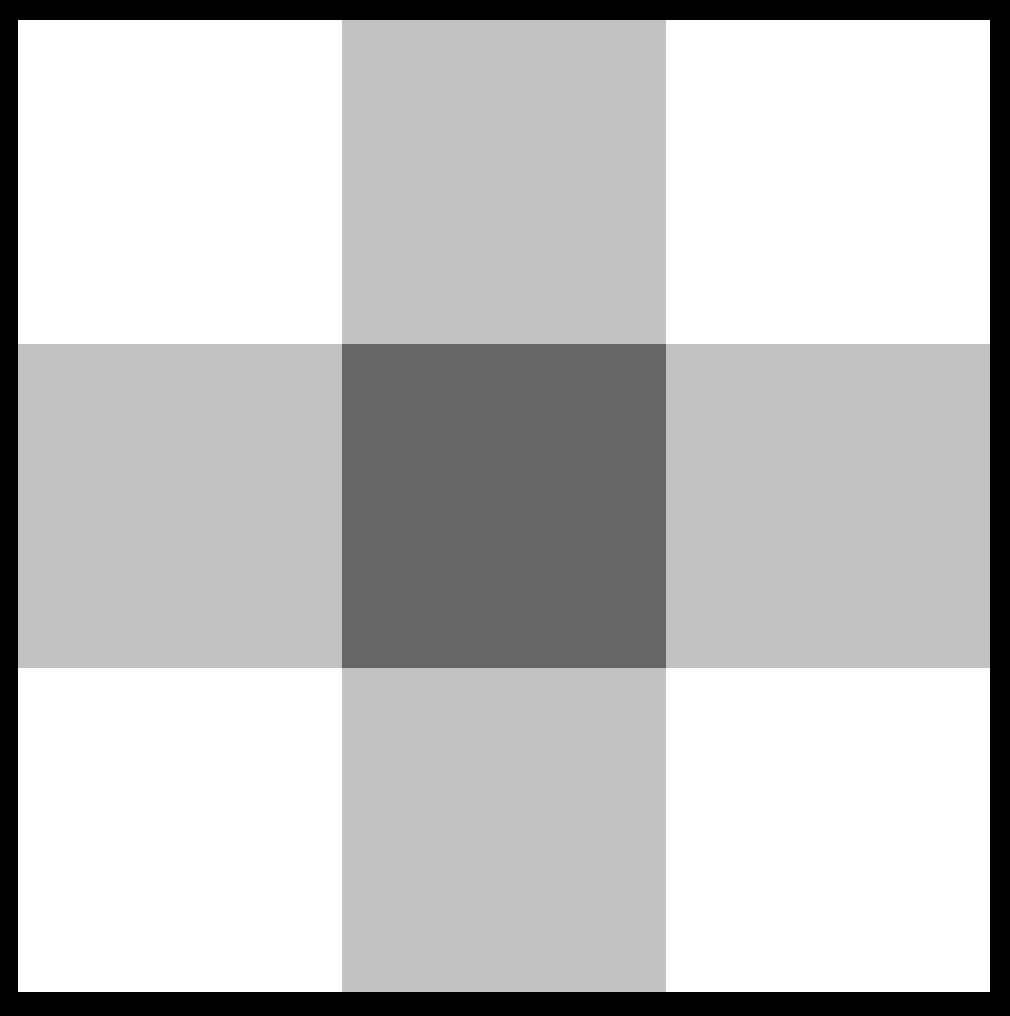
\includegraphics[width=4cm]{neighbours-4.png}
                }
                \hspace{8pt}
                \subfloat[][Sąsiedztwo ośmiospójne]{
                    \label{fig:neighbors-8}
                    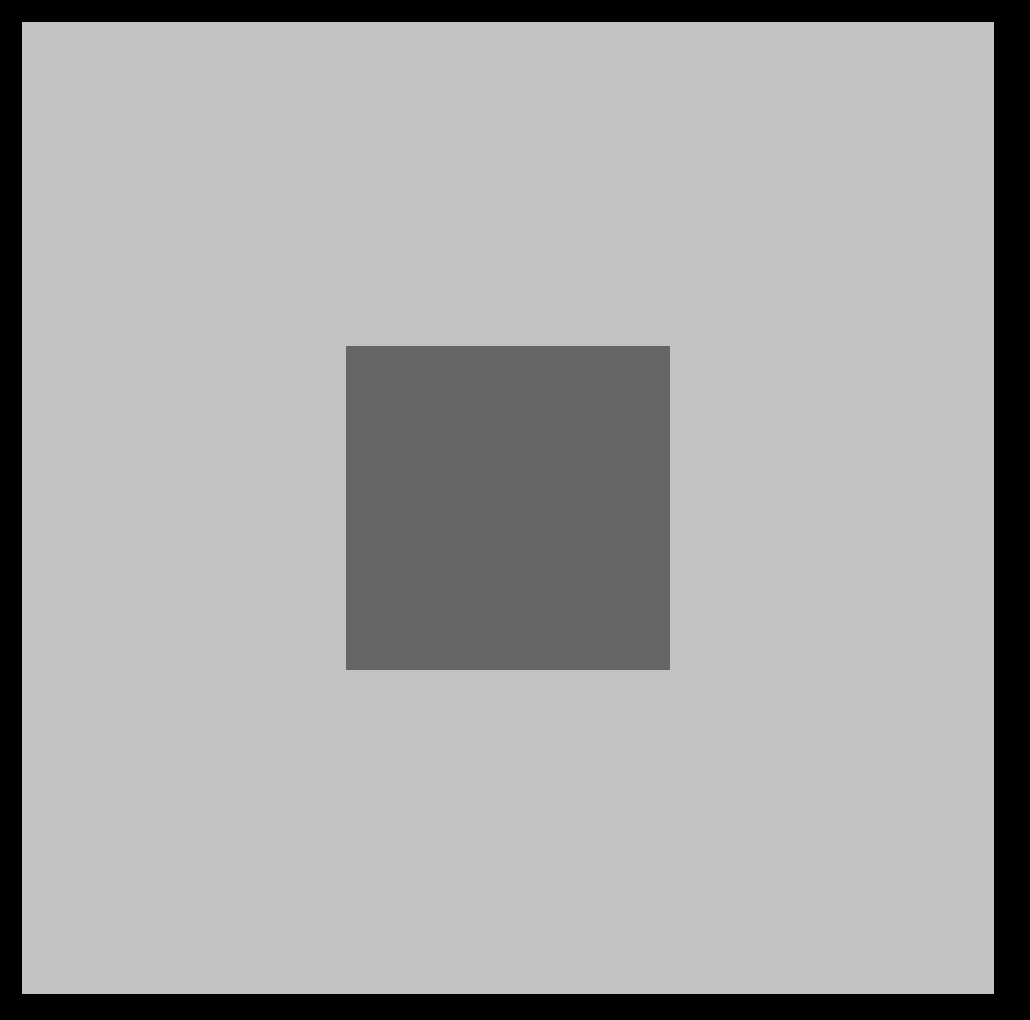
\includegraphics[width=4cm]{neighbours-8.png}
                }

                \caption[Rodzaje sąsiedztwa]
                {Rodzaje sąsiedztwa pikseli}
                \label{fig:neighbors}
            \end{figure}

            Długość krawędzi $E_{ij}$ łączącej piksele reprezentowane przez wierzchołki $V_i$ oraz $V_j$ wyznaczana jest
            na podstawie różnicy wartości łącznej intensywności wszystkich kanałów \textit{RGB}, opisanej wzorem
            \ref{eqt:pixeldiff}, w którym $p_i$ oznacza posczególny piksel, a $p_i^r$, $p_i^g$, $p_i^b$ jego składowe.
            Taki sposób doboru długości krawędzi pozwoli ,,zachęcić'' mrówki do poruszania się, a co za tym idzie
            odkładania śladu feromonowego, po ścieżkach łączących piksele podobne, jeśli ich długość będzie odwrotnie
            proporcjonalna do różnicy intensywności, lub zróżnicowane, jeśli długość będzie proporcjonalna do różnicy.

            \begin{equation}\label{eqt:pixeldiff}
                \Delta p_{ij} = \frac{(p_i^r - p_j^r)^2 + (p_i^g - p_j^g)^2 + (p_i^b - p_j^b)^2}{255^2 \cdot 3}
            \end{equation}

            Tak utworzony graf, nie jest grafem pełnym. Oznacza to, że reprezentowany przez niego problem nie jest
            równoważny z klasycznym problemem komiwojażera. Kolejną trudnością występującą w przypadku chęci
            sprowadzenia tego zadania do \textit{TSP} jest liczba wierzchołków grafu. Poszukiwanie cykli Hamiltona dla
            grafu o $w \times h$ wierzchołkach jest co najmniej nieefektywne, gdyż wartość iloczynu szerokości $w$ oraz
            wysokości $h$ nawet dla małych obrazów osiąga bardzo duże wartości.

            W związku z tym, w celu zastosowania powyższej metody, wprowadzono pewne zmiany w sposobie uruchamiania i
            działania systemu mrówkowego. Najważniejsza z nich polega na zrezygnowaniu z kończenia przez mrówki pełnych
            cykli. Zamiast tego, liczba wykonywanych kroków w każdej iteracji algorytmu jest kolejnym parametrem
            algorytmu. W celu usprawnienia działania algorytmu dla obrazów o dużych rozmiarach, wprowadzono
            możliwość generowania grafu dla obrazu przeskalowanego oraz ponownego przeskalowania macierzy maskującej do
            oryginalnych rozmiarów $w \times h$.

            Wymusiło to również adaptację części reguł aktualizacji śladu feromonowego. Ponieważ uzyskany graf nie jest
            pełny, istnieje ryzyko przedwczesnego utknięcia mrówki w pozycji, z której nie może wykonać kolejnego kroku,
            gdyż wszystkie sąsiadujące wierzchołki zostały już odwiedzone. Trasa mrówki która nie zdołała wykonać
            zadanej liczby kroków będzie krótsza od tras pozostałych mrówek, co przełoży się na jej niesłuszne
            faworyzowanie. Powyższym niebezpieczeństwem są dotknięte systemy, które w regule aktualizacji śladu
            wykorzystują długość całej trasy. Należy do nich cykliczny model systemu mrówkowego (\textit{Ant-cycle}),
            system mrowiskowy oraz system max-min. W związku z powyższym, zdecydowano się uwzględnić możliwość
            wystąpienia niepełnych ścieżek i do równań wprowadzono czynnik skalujący dystans trasy do zadanej liczby
            kroków. Przykładowo, wzór modelu cyklicznego opisanego wzorem \ref{eqt:pheromone-cycle} ma postać:

            \begin{equation}\label{eqt:pheromone-cycle-adjusted}
                \Delta\tau_{ij}(t, t + n) = \sum_{k=1}^m \left\{
                        \begin{matrix}
                            \frac{Q}{||L^k|| \cdot \frac{|L^k|}{N}} & (i, j) \in L_k\\
                            0 & w\ przeciwnym\ wypadku
                        \end{matrix}
                    \right.
            \end{equation}

            gdzie $|L^k|$ oznacza liczbę kroków trasy $L^k$, a $N$ docelową liczbę kroków zadaną podczas uruchamiania
            algorytmu.

            % ŚLAD FEROMONOWY -> MACIERZ MASKUJĄCA
            Ponieważ macierz maskująca musi posiadać wymiary identyczne z obrazem wejściowym, współczynnik na pozycji
            $x, y$ musi odpowiadać pikselowi $p_{ij}$. W celu wyznaczenia wartości elementów macierzy, które decydują o
            liczbie bitów, które zostaną zastąpione bitami ukrywanej wiadomości, obliczając wartość współczynnika
            $K_{xy}$ należy rozpatrzeć wszystkie krawędzie wychodzące z wierzchołka grafu, któremu odpowiada piksel
            $p_{ij}$.

            Dylematem, który powstał podczas opracowywania powyższej metody jest decyzja dotycząca zależności pomiędzy
            różnicami sąsiadujących pikseli $\Delta p_{ij}$ a długością krawędzi grafu. Początkowe eksperymenty wykazały
            wyższą skuteczność metody w której długości krawędzi są proporcjonalne do różnicy pomiędzy sąsiadującymi
            pikselami. Ponieważ oznacza to intensywniejsze i częstsze odkładanie feromonu na krawędziach łączących
            podobne piksele, musiało to zostać uwzględnione podczas tworzenia macierzy maskującej. Liczba bitów
            ukrywanych w danym pikselu jest zatem odwrotnie proporcjonalna do natężenia śladu feromonowego.

            W związku z powyższym, wartość $K_{xy}$ określa wzór \ref{eqt:vertex-based-converter-matrix}. $A_i$ oznacza
            zbiór pikseli sąsiadujących z pikselem $i$.

            \begin{equation}\label{eqt:vertex-based-converter-matrix}
                K_{xy} = 255 \cdot (1 - \frac{\sum_{j \in A_i} \tau_{ij}}{|A_i|})
            \end{equation}

            Rysunek \ref{fig:method-vis-vertex} przedstawia obraz wejściowy, na który nałożono wartości długości
            krawędzi związanych z konkretnymi pikselami.

            \begin{figure}
                \centering
                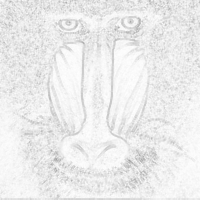
\includegraphics{method/spatial_conv.png}
                \caption{Wizualizacja grafu tworzonego metodą opartą na wierzchołkach. Jaśniejsze piksele odpowiadają wierzchołkom, do których prowadzą krótsze krawędzie}
                \label{fig:method-vis-vertex}
            \end{figure}
        }

        % METODA OPARTA O KRAWĘDZIE
        \subsection{Metoda oparta na krawędziach}\label{subsec:edge-method}
        {
            Drugim zaproponowanym podejściem jest budowanie grafu zaczynając od krawędzi. Pierwszym krokiem jego budowy
            jest podział obrazu wejściowego na ustaloną liczbę segmentów, znacznie mniejszą niż liczbę pikseli
            bitmapy. Każdy segment obrazu jest reprezentowany przez jedną krawędź grafu. Jej długość jest uzależniona od
            wariancji wszystkich pikseli należących do segmentu przez nią opisaną. Podobnie jak w przypadku konstrukcji
            grafu na podstawie wierzchołków, długość krawędzi może być wprost lub odwrotnie proporcjonalna do wartości
            wybranej miary, w tym przypadku wariancji. Uzasadnieniem wyboru wariancji jako miary opisującej każdy z
            segmentów, jest jej zdolność wyrażenia stopnia odchyleń pikseli do niego należących. Segmenty znajdujące się
            w złożonych obszarach obrazu będą posiadać wyższą wariancję.

            Następnie, z uzyskanych krawędzi tworzony jest graf pełny. Aby było to możliwe, konieczne jest spełnienie
            warunku \ref{eqt:edge-based-converter-cond}. Z tego względu, zaimplementowany algorytm jako parametr
            wejściowy przyjmuje jedynie docelową liczbę węzłów $|V|$, a liczba krawędzi $|E|$, a co za tym idzie
            segmentów obrazu, jest wyznaczana automatycznie.

            \begin{equation}\label{eqt:edge-based-converter-cond}
                |E| = \frac{|V| \cdot (|V| - 1)}{2}
            \end{equation}

            Kolejno, graf zostaje wykorzystany przez system mrówkowy. Zadanie, które jest postawione przed wirtualnymi
            mrówkami można interpretować następująco: spośród $|E|$ wszystkich krawędzi, wskaż te które pozwolą
            na ukrycie informacji w najbardziej złożonych obszarach obrazu. Jest to zadanie równoważne z problemem
            komiwojażera, przez co nie muszą być wprowadzane żadne modyfikacje algorytmu tak jak to miało miejsce w
            metodzie opartej na przekształceniu pikseli w wierzchołki grafu.

            Uzyskany ślad feromonowy przypisuje wartość liczbową każdej z krawędzi. Aby na jego podstawie uzyskać
            macierz maskującą, należy nanieść na piksele należące do segmentu $i$ wartość feromonu związaną z krawędzią
            $E_i$. Ponieważ każdy piksel jest przypisany do dokładnie jednego segmentu, wyznaczenie wartości macierzy
            maskującej nie stanowi problemu.

            % WYBRANE METODY SEGMENTACJI
            Implementacja powyższej metody jest nierozerwalnie związana z podziałem obrazu na zadaną liczbę segmentów.
            Wybór techniki nie jest wyborem oczywistym, gdyż istnieje bardzo wiele sposobów, na jakie można takiego
            podziału dokonać. W związku z powyższym, zdecydowano się wykorzystać trzy różne metody, a następnie porównać
            ich wyniki. Do wykorzystanych metod należą poniżej opisane.

            \begin{enumerate}
                \item Podział obrazu na pewną liczbę nienachodzących na siebie prostokątów w osi $x$ i $y$. Konieczny
                jest wybór takiej liczby podziałów $S_x$ i $S_y$ w osiach $x$ oraz $y$, aby ich iloczyn był równy $|E|$.
                W przeciwnym razie, zbudowanie grafu będzie niemożliwe.

                Zaletą tej metody jest jej prostota i intuicyjność, lecz ma również kilka wad. W przypadku, w którym
                wymiary bitmapy $w$ i $h$ nie są całkowicie podzielne przez $S_x$ oraz $S_y$, konieczne jest zwiększenie
                segmentów znajdujących się na końcach utworzonych wierszy i kolumn. Inną wadą są jednolite krawędzie
                podziałów -- co może przełożyć się na wyraźną różnicę jakości obrazu pomiędzy sąsiadującymi segmentami.
                Rysunek \ref{fig:method-vis-window} przedstawia wizualizację podziału obrazu powyższą metodą.

                \begin{figure}
                    \centering
                    
\includegraphics{method/window_conv.png}
                    \caption{Wizualizacja grafu tworzonego metodą opartą na podziale obrazu na nienachodzące prostokąty}
                    \label{fig:method-vis-window}
                \end{figure}

                \item Segmentację obrazu można również przeprowadzić wykorzystując algorytmy grupujące. Jednym z nich
                jest \textit{k-średnich}. Jego zastosowanie pozwala na podzielenie danych wejściowych na zadaną liczbę
                $k$ group elementów w sposób minimalizujący odległości pomiędzy elementami należącymi do tej samej grupy
                \cite{MacQueen1967SomeMF}. Algorytm pozwala na grupowanie obserwacji wielowymiarowych, lecz w tym
                przypadku zdecydowano się opisać każdy z pikseli tylko jednym atrybutem -- wariancją jego ośmiu
                najbliższych sąsiadów. Ponieważ grupowanie nie bierze pod uwagę przestrzennego położenia pikseli,
                piksele należące do tej samej grupy niekoniecznie muszą do siebie przylegać. Na rysunku
                \ref{fig:method-vis-kmeans} przedstawiono przykład podziału obrazu na zadaną liczbę grup.

                \begin{figure}
                    \centering
                    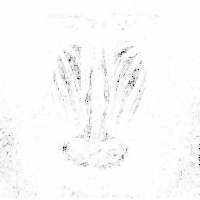
\includegraphics{method/kmeans_conv.png}
                    \caption{Wizualizacja grafu tworzonego metodą opartą na podziale obrazu przy użyciu algorytmu k-średnich}
                    \label{fig:method-vis-kmeans}
                \end{figure}

                \item Ostatnią wykorzystaną metodą segmentacji obrazu jest podział na superpiksele (ang.
                \textit{superpixels}). Superpiksele są grupami pikseli, które cechują zbliżone wartości składowych w
                przestrzeni barw. Zastosowany algorytm \textit{SLIC} polega z przestrzeni
                \textit{CIELAB} \cite{Achanta2012SLICSC}. Popularność superpikseli w dziedzinie przetwarzania obrazów
                stale rośnie, gdyż pozwalają na uchwycenie najważniejszych cech obrazu przy znacznej redukcji jego
                reprezentacji. To z kolej przekłada się na krótszy czas pracy algorytmów przetwarzania obrazu. Ich
                zastosowania można znaleźć rozwiązywaniu problemów identyfikacji i wyodrębniania obiektów. W
                przeciwieństwie do algorytmu \textit{k-means}, uzyskane grupy pikseli są spójne. Rysunek
                \ref{fig:method-vis-super} przedstawia wizualizację podziału obrazu powyższą metodą.

                \begin{figure}
                    \centering
                    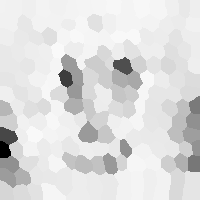
\includegraphics{method/superpixel_conv.png}
                    \caption{Wizualizacja grafu tworzonego metodą opartą na podziale obrazu na superpiksele}
                    \label{fig:method-vis-super}
                \end{figure}
            \end{enumerate}
        }
    }
}

% ALG MRÓWKOWE W STEGANOGRAFII
% Zhao2021AntCO file:///Users/grzegorzkazana/Desktop/Stegano_Ant/Ant%20colony%20optimization%20with%20horizontal%20and%20vertical%20crossover%20search%20Fundamental%20visions%20for%20multi-thres.image%20segmentation.pdf
% Mohadeseh2013ANT file:///Users/grzegorzkazana/Desktop/Stegano_Ant/A%20Novel%20Technique%20for%20Steganography%20Method%20Based%20on.pdf
% Khan2018AntCO file:///Users/grzegorzkazana/Desktop/Stegano_Ant/Ant%20Colony%20Optimization%20ACO%20based%20Data%20Hiding%20in%20Image%20Complex%20Region.pdf
% ZghaerACOStegEN file:///Users/grzegorzkazana/Desktop/Stegano_Ant/Ant%20Colony%20Optimization%20To%20Enhance%20Image%20Steganography.pdf
% Priya2018HIGHCA file:///Users/grzegorzkazana/Desktop/Stegano_Ant/HIGH%20CAPACITY%20AND%20OPTIMIZED%20IMAGE%20STEGANOGRAPHY%20TECHNIQUE%20BASED%20ON%20ANT%20COLONY%20OPTIMIZATION%20ALGORITHM.pdf
% ElEmam2013NewSA file:///Users/grzegorzkazana/Desktop/Stegano_Ant/New%20steganography%20algorithm%20to%20conceal%20a%20large%20amount%20of%20secret%20message%20using%20hybrid%20adaptive%20neural.pdf
